\documentclass{article}

\usepackage{amsmath} % For gather and other math environments
\usepackage{setspace} % For double spacing
\usepackage{mathtools} % amsmath extensions
\usepackage{amsfonts} % math fonts
\usepackage{graphicx} % for images
\usepackage{listings} % for code blocks
\usepackage{pgfplots} % for plotting function
\usepackage{booktabs} % for tables
\usepackage{float}

\usepackage[a4paper, margin=3.17cm]{geometry}

\graphicspath{{ ./images/ }}

% notes:
% https://hudsonthames.org/caveats-in-calibrating-the-ou-process/
% closed-form OU solution, do this youself tho: https://fxpaul.wordpress.com/2011/05/27/closed-form-solution-of-modified-ornstein-uhlenbeck-process/
% interesting, close form solution to SDE for trading: https://arxiv.org/pdf/2003.10502
% https://github.com/david-alber/Pairs-Trading-as-application-to-the-Ornstein-Uhlenbeck-Process

% process calibration:
% https://dr.lib.iastate.edu/entities/publication/bf86f169-61a5-44fc-8f2f-d8e6cd7e103a

% out-of-sample performance of an OU process:
% https://onlinelibrary.wiley.com/doi/abs/10.1002/for.2720

% rly interesting:
% https://github.com/david-alber/Pairs-Trading-as-application-to-the-Ornstein-Uhlenbeck-Process/blob/master/Report%2BPoster/Pairs_Trading_Doc.pdf

% dickey fuller:
% https://www.youtube.com/watch?v=1opjnegd_hA

% source for unit-root testing (part of Engle Granger Test):
% https://pages.stern.nyu.edu/~churvich/Forecasting/Handouts/UnitRoot.pdf

% very good video on DF and ADF tests, doesn't actually really explain how to do them:
% https://www.youtube.com/watch?v=T5BhGv742j4


% notes on stochastic processes and SDEs
% https://math.nyu.edu/~goodman/teaching/DerivSec10/notes/week6.pdf
% https://planetmath.org/analyticsolutiontoornsteinuhlenbecksde
% https://geelon.github.io/assets/talks/sde.pdf
% https://ludwigwinkler.github.io/blog/SolvingSDEs/

\begin{document}

\begin{titlepage}
    \vspace*{\fill}
    \vspace*{-4cm}
    \begin{center}
        \huge \textbf { Ornstein Uhlenbeck Process Statistical Arbitrage and Cointegration on Equity Markets } \\
        \vspace{0.5cm}
        \Large \textit { by Filip Toth }
    \end{center}
    \vspace*{\fill}
    \begin{center}
        \large \textit {A Mathematical Exploration for IB Math: Applications \& Interpretations HL}
    \end{center}
\end{titlepage}

\begin{spacing}{2.0}
\section{Brownian Motion and the Wiener Process}

Consider a stochastic process, where per each iteration, we add a $\Delta$ to the previous value,
this $\Delta$ is distributed by a normal distribution with a $mu$ of zero, and these are independent
stochastic events this is called the Wiener process. In discrete time, we can define the Wiener process
with the following equation
\begin{gather*}
    W_{t + 1} = W_{t} + \mathcal{N}(0, \sigma^{2})
\end{gather*}
Where $W_{t + 1}$ is the next value of the process (under discrete time), $\mathcal{N}(0, \sigma^{2})$
is a normally distributed drift variable with the variance $\sigma^{2}$.

Intuitively, the expected value, i.e. the limit of this process as it approaches infinity, should
be zero, since the normal distribution is symmetric. (maybe prove this? Using a limits on the $\mathbb{E}[W]$ and the normal dist)

The spread of the Wiener process grows at a rate of $\sigma_{t} = \sigma \sqrt{t}$, due to each timestep adding additional compounded uncertainty.

Here's an example of a Wiener process with $W_{0} = 0$ and $\sigma^{2} = 1$:
\begin{center}
    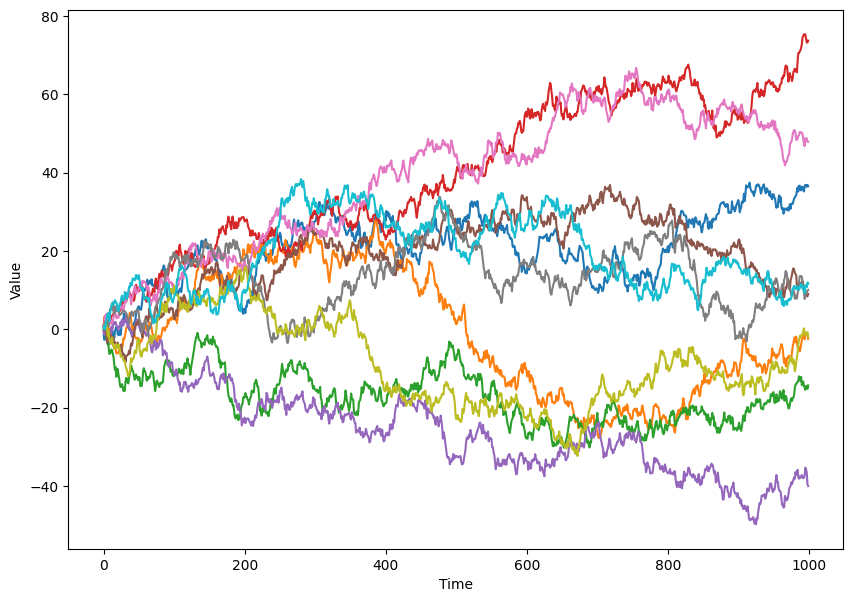
\includegraphics[scale=0.35]{./images/wiener.png}
\end{center}
In the diagram, we can clearly observe that the the variance of the Wiener process gets larger as the time progresses.

The wiener process is crucial and has many financial applications, for example, equity prices under the assumption of the efficient
market hypothesis follow a purely-stochastic Wiener process. This although disregards stochastic drift, which applies directional
pressure on equity prices, i.e., the Wiener process is market-agnostic, and applies to equity which do not follow the upward trend
of the market due to the positive risk-free rate.


\section{Ornstein-Uhlenbeck Process}

\subsection{Deriving a Mean Reversion Mechanism}

But what if we don't want the variance of the process to get larger as time progresses? We call these processes mean-reverting, as in they
tend to revert their values back towards the mean $\mu$. This has numerous financial applications (not to mention its applications outside
of finance), for example: statstical arbitrage, interest rate models, heston model, and mean reverting equities.

So how do we implement mean reversion? We can start by thinking about what mean reversion actually is? Mean reversion is the tendency of a
variable (or usually a stochastic process) to revert back to its long-term mean. If we consider the roots of brownian motion - physics -, we
can consider a mean-reverting term to be similar to a force pushing a particle back towards its mean; note that this doesn't happen
instantaneuously, it happens over a period of time, where the steadyness of this decay is dictated by the rate of mean-reversion, denoted as
$\theta$.

We know that an exponential function with a negative coefficient applied to the exponent will produce a function that will slowly decay.

\begin{center}
\begin{tikzpicture}
    \begin{axis}[
        axis lines = left,
        xlabel = \(x\),
        ylabel = {\(f(x)\)},
    ]
        \addplot [
            domain=0:15,
            samples=100,
            color=red,
        ] {e^(-0.4 * x)};

        \addlegendentry{$f(x) = x_{0} \cdot e^{-\theta x}$}
    \end{axis}
\end{tikzpicture}
\end{center}

But this is not exactly mean reverting, we need to adjust the function to not only have the tendency to approach zero, but rather, the function must approach
the mean. And the function must be applied from any starting point $x_{0}$. Considering that $f(0) = x_{0}$, we can adjust the function and introduce a base
term: $f(x) = x_{0}e^{-\theta x}$, this ensures the initial value is $x_{0}$, since $e^{0} = 1$. Now we have to ensure that the function converges at the mean,
not at zero. Initially, we can try to add a the mean as a constant term, such that $f(x) = \mu + x_{0}e^{-\theta x}$, but when graphing this function, we notice
that we break our first condition - the initial value of the function $f(0)$ is not equal to $x_{0}$. We have to adjust for this in the coefficient of the
exponential term. We notice that the difference between $x_0$ and $f(0)$ is equal to the mean, thus modifying the function to the following will solve our problem:

\begin{gather*}
    f(x) = \mu + (x_{0} - \theta)e^{-\theta x}
\end{gather*}

The function produces the following graph, assuming $\mu = 4$, $\theta = 0.4$ and varying the initial value $x_{0}$ to be $x_{0} \in \{8, 5, -1 \} $ for each of the
separate lines respectivelly:

\begin{center}
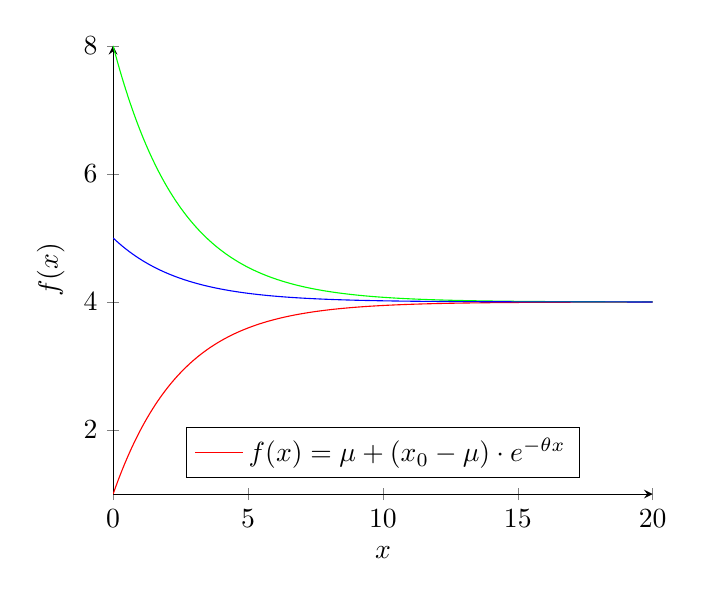
\begin{tikzpicture}
    \begin{axis}[
        axis lines = left,
        xlabel = \(x\),
        ylabel = {\(f(x)\)},
        legend style={
            at={(0.5,0.15)},
            anchor=north,
            cells={anchor=west}
        },
    ]
        \addplot [
            domain=0:20,
            samples=400,
            color=red,
        ] {4 + (1 - 4) * e^(-0.4 * x)};

        \addplot [
            domain=0:20,
            samples=400,
            color=green,
        ] {4 + (8 - 4) * e^(-0.4 * x)};

        \addplot [
            domain=0:20,
            samples=400,
            color=blue,
        ] {4 + (5 - 4) * e^(-0.4 * x)};

        \addlegendentry{$f(x) = \mu + (x_{0} - \mu) \cdot e^{-\theta x}$}
    \end{axis}
\end{tikzpicture}
\end{center}

\subsection{Differentiating for the Mean-reverting Force}

We can now think about creating a stochastic process that will take the Wiener process as a basis, but add mean-reverting properties in order to ensure
the variance stays within a certain range. Just adding a term for the brownian motion will not be enough, this would be misinterpreting the mean-reverting
effect and would be mostly useless for our purposses, thus we can't do something like:
\begin{gather*}
    X_{t} = \mu + (X_{0} - \mu) \cdot e^{-\theta t} + \sigma W_{t}
\end{gather*}
We must now calculate the tug or the actual amount by which the function changes per unit $t$. This will be necessary for our stochastic process, as they
are inherently defined in differential form (in descrete time), where the next value depends on the previous value and we simply add a modifying term, e.g.
$M_{t + 1} = M_{t} + \sigma$. We can do this by taking a simple derivative of the function. This derivative can then be thought of as the per-unit $t$ amount
of tug applied for each value above or below the mean.
\begin{gather*}
    \frac{d}{dt} \left ( \mu + \left ( X_{0} - \mu \right ) \cdot e^{-\theta t} \right ) \\
    \frac{d}{dt} \mu + \frac{d}{dt} \left ( X_{0} - \mu \right ) e^{-\theta t}
\end{gather*}
We know that the derivative of the constant $\mu$ is zero, thus we can eliminate the term. We are left with the derivative of a product, for which we can
use the product rule of differentiation: $\frac{d}{dt}x \cdot y = x'y + xy'$. In our case, the two terms are $( X_{0} - \mu )$ and $e^{-\theta t}$. The first
term is a constant that does not chage with respect to $t$, thus it will be zero. The second term can be differentiated using the chain rule.

We need to define an outer and an inner function in order to apply the chain rule, the inner function will be $e^{x}$ and the outer function will be $-\theta t$.
The $\frac{d}{dx}e^{x} = e^{x}$ is a standard differential. And the $\frac{d}{dx} -\theta x$ will simply collapse down to $-\theta$, since it's a constant that is
applied to our differentiating variable. The chain rule states:
\begin{gather*}
    \frac{d}{dx} f(g(x)) = f'(g(x)) \cdot g'(x) \\
    \frac{d}{dt} e^{-\theta x} = e^{-\theta x} \cdot (-\theta) = -\theta e^{-\theta x}
\end{gather*}
We can now revisit the prudct rule and apply it, we know that the derivative of our first term is zero, thus we can ignore the first term of the product rule.
Only leaving the following: $\frac{d}{dt}x \cdot y = xy'$, we have already calculated $y' = -\theta e^{-\theta x}$ in the previous step. Thus we can Just
multiply $-\theta e^{-\theta x}$ with $(X_{0} - \mu)$, and we get the following result for our whole derivative:
\begin{gather*}
    \frac{d}{dt} \left ( \mu + \left ( X_{0} - \mu \right ) \cdot e^{-\theta t} \right ) = (-\theta e^{-\theta x}) \cdot (X_{0} - \mu)
\end{gather*}
We can rearrange this to:
\begin{gather*}
    \frac{d}{dt} \left ( \mu + \left ( X_{0} - \mu \right ) \cdot e^{-\theta t} \right ) = -\theta (X_{0} - \mu) e^{-\theta t}
\end{gather*}
This differential desribes the mean-reverting tug applied to our brownian motion model.

\subsection{Full Naive Derivation of the OU Process}

We can now try to perform a few experiments on a naively-formulated OU (Ornstein Uhlenbeck) process. We can begin by simply adding a brownian motion to our stochastic
process, and assuming (naive step) $X_{0} = X_{t}$, since at each point, the differential will get us tug, this will mean that our $t$ is now zero.
We are left with the following stochastic process:
\begin{gather*}
    X_{t + 1} = -\theta(X_{t} - \mu)e^{-\theta \cdot 0} + W_{t} \\
    X_{t + 1} = -\theta(X_{t} - \mu)e + \mathcal{N}(0, \sigma^{2})
\end{gather*}
We can not create stochastic paths along the process and they should be mean reverting. A stochastic path (more formally called a sample path of a stochastic process) is simply
a possible outcome of running the process, esentially a random path that conforms to the process.
\begin{center}
    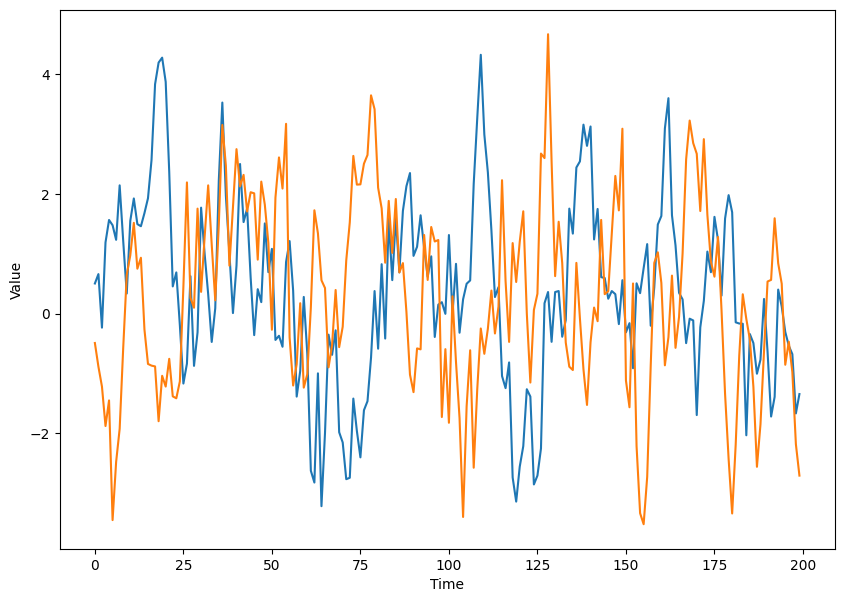
\includegraphics[scale=0.35]{./images/naive_ou.png}
\end{center}
Here we can see that the stochastic process is much more contained within a range, and is thus mean-reverting.

\subsection{Formal Derivation of the OU Process}

The Ornstein Uhlenbeck process is formally defined as a stochastic differential equation (SDE). An SDE is just a differential equation with a stochastic term.

We begin with adding a brownian motion component. A standard wiener process in its differential form is: $dX_{t} = dW_{t}$, this is pretty straight forward if you think about it,
the change in $X_{t}$ is just the change in $W_{t}$, this being a stochastic component, $dW_{t}$ will always be different, and for the sake of simplicity, we can visualize this as if
the term follows the normal distribution $dW_{t} \sim \mathcal{N}(0, \sigma^2)$, this isn't entire true because the variance of the normal distribution itself depends on $dt$,
but we will get to that later.

We now add the drift term (which we derived in a previous subchapter) $\theta(\mu - X_{t})$ (we derived it as $-\theta(X_{t} - \mu)$, but these are functionally equivalent), we can say that this drift happens
- continuously - over time t, thus can be written as $\theta(\mu - X_{t}) dt$, recall that $dt$ here represents an infinitesmal (very small) change in time $t$, thus the whole term
represents the change in the process value $X_{t}$ as we change time $t$ by an infinitesmal amount and can thus be written as $\frac{d X_{t}}{dt} = \theta(\mu - X_{t})$, but this
is just basic differential equations. We end up with:
\begin{gather*}
    dX_{t} = \theta(\mu - X_{t}) dt + dW_{t}
\end{gather*}
We also add a variable $\sigma$ to our process, not to be confused with the standard deviation, in our context, $\theta$ represents the intensity of the brownian motion (stochastic)
component. We end up with the final formal definition of the OU process:
\begin{gather*}
    dX_{t} = \theta(\mu - X_{t}) dt + \sigma dW_{t}
\end{gather*}


\section{Long-term Equilibrium Cointegration in Equity Markets}

We perform the \textbf{Two Step Engle-Granger Test} for cointegration of time series to get the cointegration coefficient. This method is widely accepted
in quantitative finance and econometrics.

But what is cointegration? Cointegration represents the level to which a linear combination
of two (or more) time series $X_{t} = \beta Y_{t}$ follows a stationary time series $I(0)$.
Or in other words, whether the linear combination has a zero long-term mean. We can take
any linear combination, such as the linear regression of $X_{t}$ on $Y_{t}$, in the next
sub-chapter, we form this regression and add an error term, the error term is esentially
formed from a linear combination of the two time series. A high cointegration coefficient
means that the two time series move in tandem with each other and that deviations in their
spread revert to the long-term mean (since the mean of the spread is zero), divergence of
spreads resulting in a zero long-term mean spread is impossible because the function is
continuous.

\subsection{Static Regression of Equity Time Series}

First, we need to determine the residuals $\hat \epsilon_{t}$ (similar to the error) of a regression between
the two time series of the prices of the equities we're analyzing. We define a linear regression $Y_{t} = \alpha + \beta X_{t} + \epsilon_{t}$.
Where $Y_{t}$ and $X_{t}$ are the $t$-th elements of the time series of the equity prices of $X$ and $Y$. And where $\alpha$ is the
intercept term (which is the mean level of $Y_{t}$ where $X_{t}$ is zero) and where $\beta$ is mean slope coefficient, i.e. the change in
the value of $Y_{t}$ per unit $X_{t}$.
We define the following intuitively or from the definition of the linear regression:
\begin{gather*}
    \beta = \frac{
        \sum_{i = 0}^{n}{(X_{i} - \mu_{X}) \cdot (Y_{i} - \mu_{Y})}
    }{
        \sum_{x \in X} (x - \mu_{X})^2
    }
    \\
    \alpha = \mu_{Y} - \beta \cdot \mu_{X}
\end{gather*}
Now we calculate the residuals $\hat \epsilon_{t}$ using the formula $\hat \epsilon_{t} = Y_{t} - (\alpha + \beta X_{t})$, which we obtain from rearranging the
terms of the linear regression equation with resduals. We can interpret these residuals as the difference (for each timestep $t$) between the actual value $X_{t}$
and the predicted value - the value of the regression solution for the parameter $t$.



\subsection{Dickey Fuller Test}

The Dickey Fuller Test or (DF Test for short) is a statistical test that tests for the stationarity of a time series, or in other words, it tests for if the
order of integration of the time series is $I(0)$. The non-augmented version of the Dickey Fuller Test is only applicable for an auto-regressive AR(1) process.
Equity spreads are widely considered to be AR(1) processes. We can define an AR(1) time series as $y_{t} = \alpha + \phi y_{t - 1} + \epsilon_{t}$, where $\alpha$ is
the constant shift term, $\phi y_{t - 1}$ is the autoregressive term where $\phi$ is a coefficient denoting how strongly the previous value of the time series
affects the current value at time $t$, and $\epsilon_{t}$ (not to be confused with the residuals from our regression model) denotes a random error term, which IS
assumed to be white noise $\epsilon_{t} \sim \mathcal{N}(0, \sigma^2)$. Now we can define the hypotheses for the DF Test.
\begin{gather*}
    H_{0} : \phi = 1 \\
    H_{1} : \phi < 1
\end{gather*}
Where the null hypothesis denotes that the process is non-stationary and the alternative hypothesis indicates that the process is stationary. We could simply use a t-test
to see if a $\hat \phi$ estimator is statistically significant, and based on that reject or fail to reject the null hypothesis of the DF Test. But the t-test is inapplicable
in models where the central limit theorem doesn't hold true (because the $\epsilon$ values of the process are not independent and identically distributed), thus we need to use the
DF test. First, we transform our original time series expression in as a differencing equation. Note that we also rewrite the $y_{t} - y_{t - 1}$ as $\Delta y_{t}$.
\begin{gather*}
    y_{t} = \alpha + \phi y_{t - 1} + \epsilon_{t} \\
    y_{t} - y_{t - 1} = \alpha + \phi y_{t - 1} - y_{t - 1} + \epsilon_{t} \\
    \Delta y_{t} = \alpha + y_{t - 1} (\phi - 1) + \epsilon_{t}
\end{gather*}
For the sake of simplicity, we introduce $\delta$ instead of $(\phi - 1)$. We can simplify our express to $\Delta y_{t} = \alpha + \delta y_{t - 1} + \epsilon_{t}$, which is
the standard form you'll find in most literature on the DF Test. Our hypotheses remain and can be rewritten in terms of $\delta$ instead of $\phi$.
\begin{gather*}
    H_{0} : \delta = 0 \\
    H_{1} : \delta < 0
\end{gather*}
We apply an Ordinary Least Squares linear regression to find the estimator $\hat \delta$, this is the p-value for our test and we compare it against our hypotheses. But in our case,
we this won't be rigorous enough since we didn't account for autocorrelation (In our case, this means that previous values have some sort of effect on the current value $y_{t}$ in our
time series) properties of financial time series, to remedy this and correctly account for autocorrelation, we use the Augmented Dickey Fuller Test or ADF for short.

\subsection{Augmented Dickey Fuller Test}

This is an extension of the Dickey Fuller Test that correctly accounts for autocorrelation between consecutive values of the time series and is also extended to the autoregressive
AR(p) process; it tests whether a time series of the order of integration $I(p)$ is stationary and for the presence of a unit root (which is a prerequisite of non-stationarity).
In the ADF test, our hypotheses stay the same.
\begin{gather*}
    H_{0} : \delta = 0 \text{ $\rightarrow$ non-stationary, unit root} \\
    H_{1} : \delta < 0 \text{ $\rightarrow$ stationary, no unit root}
\end{gather*}
We need to add lags to our expression to account for autocorrelation. We can model autocorrelation as some coefficient applied on some previous value of the time series also being
accounted in the value of the time series at $t$. Considering we add two lags to account for autocorrelation between the current value $y_{t}$ and values $y_{t - 1}$ and $y_{t - 2}$,
our expression will intuitively become $\Delta y_{t} = \alpha + y_{t - 1} (\phi - 1) + \beta_{1}(\Delta y_{t - 1}) + \beta_{2}(\Delta y_{t - 2}) + \epsilon_{t}$. Where the betas $\beta_{1}$
are our coefficients onf the lagged differences. We also define $p$ to be the number of lags we include, this value is automatically optimized in various statistical application
programming interfaces (APIs) and one can use various Bayesian estimation methods to get the optimal $p$ value, or one can perform a t-test (or an F-test when testing for the significance
of multiple variables) and keep adding lagged differences (thus increasing $p$) until the addition is no longer statistically significant. Our expression can be generalized in the
following form:
\begin{gather*}
    \Delta y_{t} = \alpha \delta y_{t - 1} + \sum_{i = 1}^{p} \beta_{i} \Delta y_{t - 1} + \epsilon_{t}
\end{gather*}
Now that we have this equation, we can do an Ordinary Least Squares regression (in its multiple linear regression form, since we have multiple regressors) to find
$\alpha, \delta, \beta_{1}, \beta_{2}, \dots, \beta_{p}$, we then use the $\delta$ value as the final p-value for the Augmented Dickey Fuller Test.

\subsection{Performing the Two-Step Engle Granger Test on Equity Prices}

We now perform the two-step engle granger test on 78 mature stocks from the selected from NADSAQ-100 index from Janurary 1st 2014 to January 1st 2024. We pair every stock with every other
stock resulting in $78^2 = 6084$ pairs, for each of these pairs we perform an OLS regression and get the residual values (as described in subsection 1) and then perform the Augmented Dickey
Fuller Test using the 'statsmodels' library. We extract the p-values of the test and end up with the following heatmap:
\begin{center}
    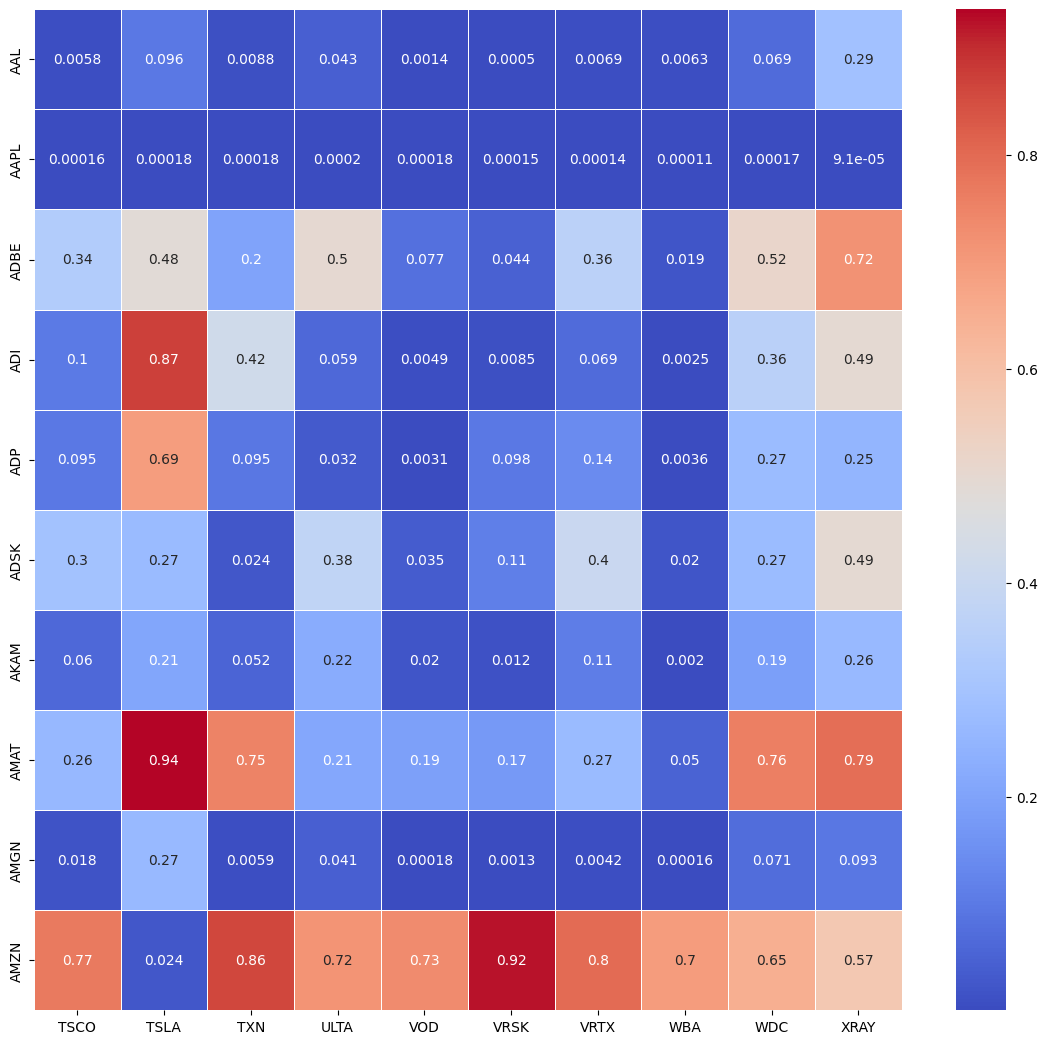
\includegraphics[scale=0.45]{./images/cointegration.png}
\end{center}
Only 100 pairs are displayed as the complete 78x78 heatmap is too large to present here.

We now select 10 of the most cointegrated (lowest p-values) equity pairs to further examine, the ten most cointegrated pairs were, in descending order of cointegration, we observe
that most of the equity pairs with very heavy cointegration have AAPL (Apple Inc.) as the base stock, this is interesting as AAPL has heavily outperformed even the growth-heavy
NASDAQ, thus this should create a larger spread between most other stocks, suggesting limitations of our test.

\begin{table}[H]
    \centering
    \begin{tabular}{|c|c|c|}
        \hline
        \textbf{Stock 1 Ticker} & \textbf{Stock 2 Ticker} & \textbf{ADF P-Value} \\ \hline
        AAPL & XRAY & 9.104296439449678e-05 \\ \hline
        AAPL & WBA & 0.00011254543577701014 \\ \hline
        AAPL & VRTX & 0.00014280647279306093 \\ \hline
        AAPL & VRSK & 0.00015429781044445213 \\ \hline
        AMGN & WBA & 0.00016469559752946386 \\ \hline
        AAPL & TSCO & 0.00016489122300362627 \\ \hline
        AAPL & WDC & 0.0001652537550668745 \\ \hline
        AAPL & TSLA & 0.00017722866444703876 \\ \hline
        AMGN & VOD & 0.00018081206670114813 \\ \hline
        AAPL & TXN & 0.00018223283943511726 \\ \hline
    \end{tabular}
\end{table}

For reference, we can plot the residuals of the initial regression of a select heavily cointegrated
pair and a non-cointegrated pair to better visualize the idea of cointegration.

\begin{figure}[H]
    \centering
    \begin{minipage}{0.48\textwidth}
        \centering
        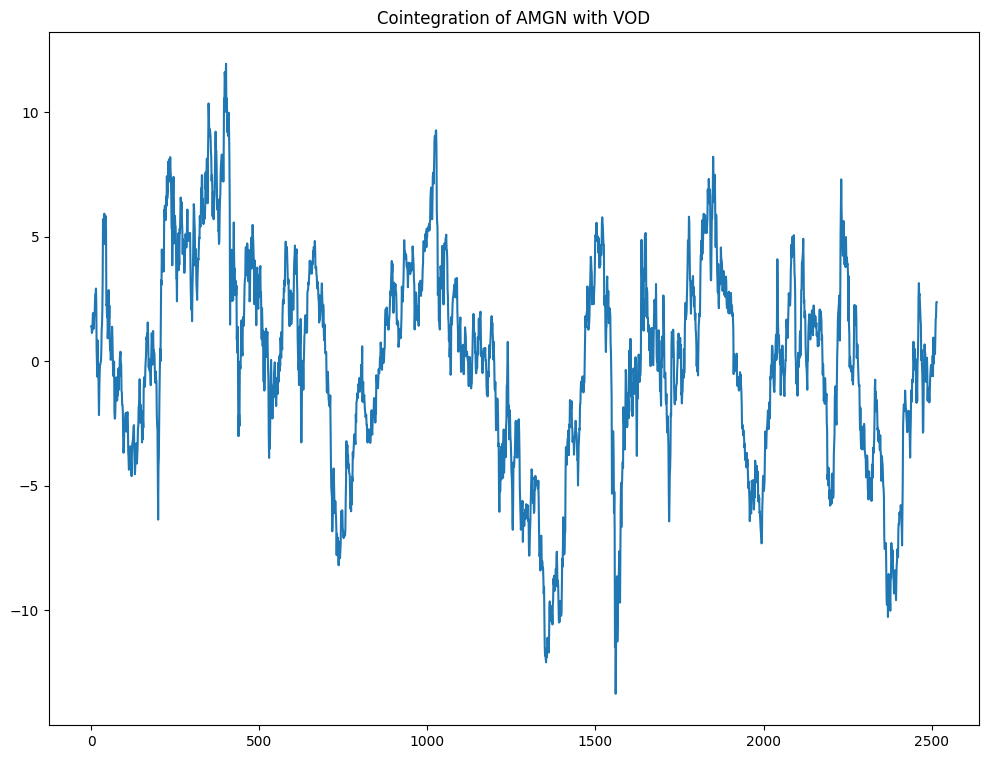
\includegraphics[width=\textwidth]{./images/amgn_vod_cointegration.png}
        \caption{AMGN, VOD, p-value: 0.000181}
    \end{minipage}
    \hfill
    \begin{minipage}{0.48\textwidth}
        \centering
        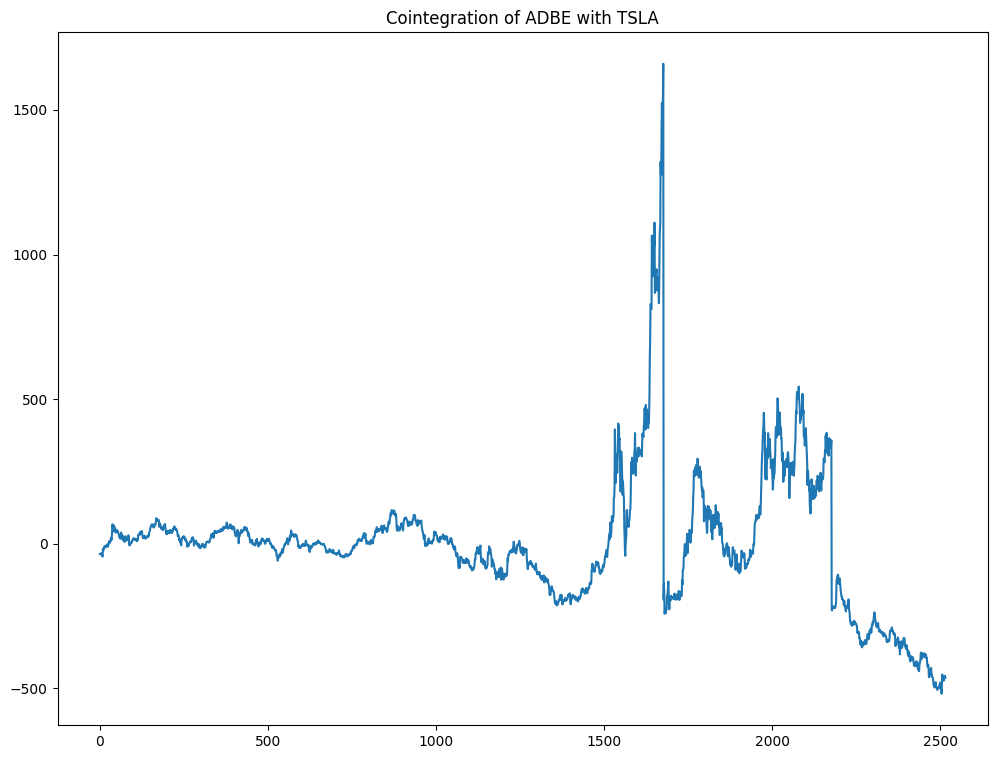
\includegraphics[width=\textwidth]{./images/adbe_tsla_cointegration.png}
        \caption{ADBE, TSLA, p-value: 0.484251}
    \end{minipage}
\end{figure}

\subsection{Engle Granger Residuals vs Equity Spreads}

If we plot the residuals of AMGN and VOD, we can observe that the resultant time series clearly follows an OU process (or a time-discrete AR(1) time series), as is also indicated
by the test we performed, but if we plot the equity spreads (values of stock 1 minues values of stock 2), we observe a different pattern, indicating that our model is still incomplete
and that OLS residuals might not give us the full picture. Let's examine the difference between the graph of the residuals and the graph of the spreads:

\begin{figure}[H]
    \centering
    \begin{minipage}{0.48\textwidth}
        \centering
        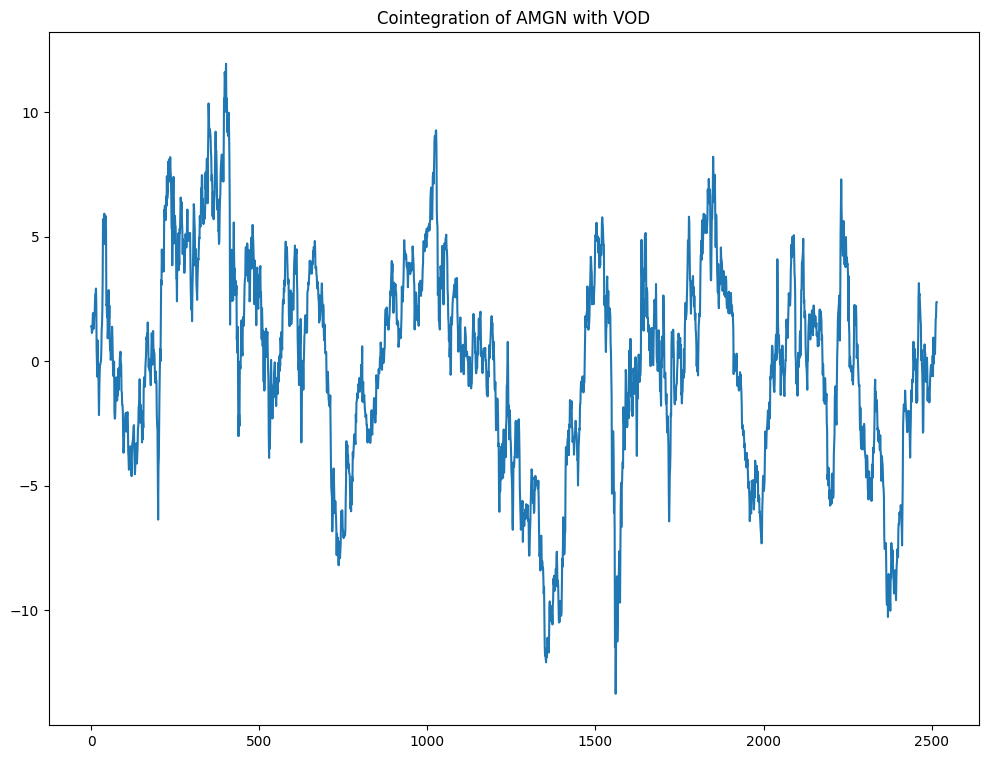
\includegraphics[width=\textwidth]{./images/amgn_vod_cointegration.png}
        \caption{AMGN-VOD cointegration regression residuals}
    \end{minipage}
    \hfill
    \begin{minipage}{0.48\textwidth}
        \centering
        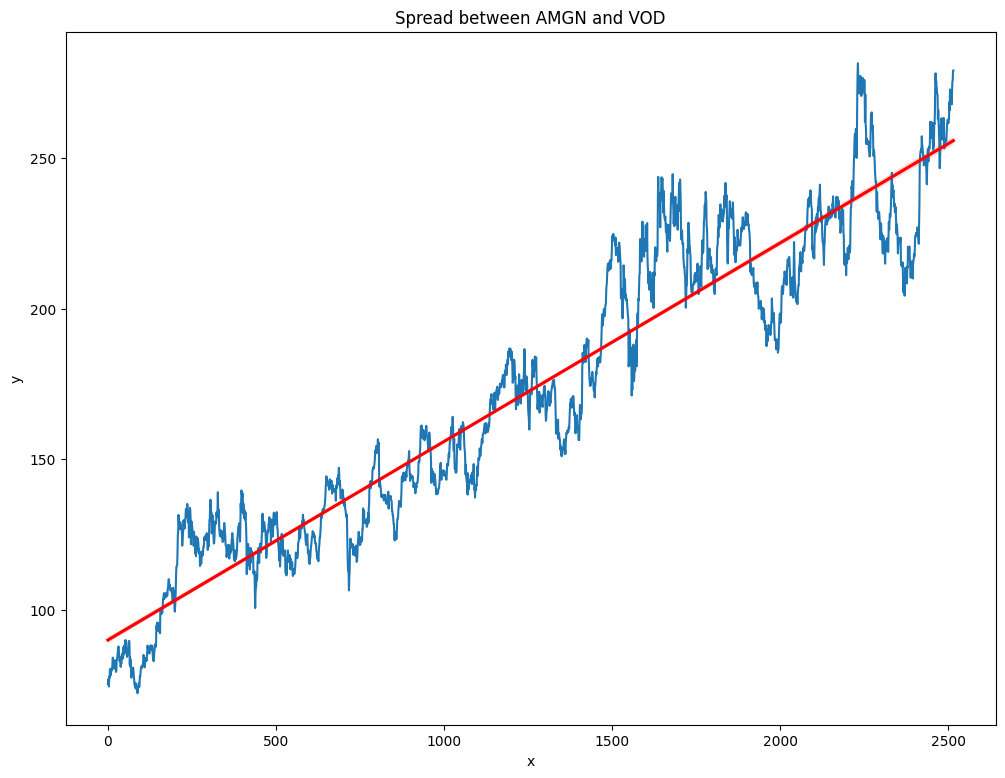
\includegraphics[width=\textwidth]{./images/spread_amgn_vod.png}
        \caption{AMGN-VOD spread with line of best fit}
    \end{minipage}
\end{figure}

We can see that the cointegration esentially disregards deterministic drift in the spreads (deterministic drift is esentially the non-stochastic trend). This makes sense if you think
about our test methodology, we defined an OLS linear regression between two stock price time series and then we used to residuals to perform the stationarity test, our graph just
shows the residuals at each time step. A residual is just the difference between the what the regression model predicts (using a standard linear equation model $y = \beta x + \alpha$)
and the actual value of the time series.

Our Ornstein Uhlenbeck model resembles the residuals and not the actual spreads, it doesn't yet account for deterministic drift.

\section{Fitting the Ornstein Uhlenbeck Process to our Data}

There are two ways you can calibrate an Ornstein Uhlenbeck process for a particular dataset. Either using a simple OLS regression for the OU parameters ($\theta$, $\sigma$, $\mu$), or
you can use a much more rigorous technique that yields better results, called: Maximum Likelyhood Estimation (MLE), while if this weren't a Math IA, I would use MLE (due to there already
being pre-existing implementation and it being fairly easy to understand, just requires basic multivariable calculus), we do not have the capacity to explain MLE in this IA, additionally,
OLS parameter estimation is frequently used in Quant Finance, despite it's obvious limitations. The first step is obtaining a formal solution to the OU stochastic differential equation (SDE).

\subsection{Formal Analytical Solution to the OU SDE}

We start with the OU SDE we derived in a previously, and we expand the deterministic drift term.
\begin{gather*}
    dX_{t} = \theta (\mu - X_{t})dt + \sigma dW_{t} \\
    dX_{t} = \theta \mu dt - \theta X_{t} dt + \sigma dW_{t}
\end{gather*}
Looking at the deterministic part of our SDE $dX_{t} = \theta \mu dt - \theta X_{t} dt$, we notice that we need to simplify this ordinary differential equation (ODE) and
find an integrating factor. An integrating dactor is given by the following: $I(x) = e^{\int P(x) \, dx}$, where $P(x)$ is defined by the standard form of a first-order ODE:
$\frac{dx}{dy} + P(x) y = Q(x)$, which we can fit to our deterministic ODE:
\begin{gather*}
    \frac{dX_{t}}{dt} = \theta \mu - \theta X_{t} \\
    \frac{dX_{t}}{dt} + \theta X_{t} = \theta \mu
\end{gather*}
where ${P(x) = \theta}$ and $Q(x) = \theta \mu$, we can now use the above-mentioned formula to find the integrating factor, $I(t) = e^{\int P(t) \, dx}$ (notice that
we switch to $t$ since $dt$ is our differential and not $dx$). Subce $\theta$ is a constant, we can easily evaluate the integral $\int \theta \, dt = \theta t + C$,
thus our integrating factor becomes: $I(t) = e^{\theta t}$, notice that we deliberately ignore the constant term $C$. Now, going back to our SDE, we can apply our
integrating factor.
\begin{gather*}
    dX_{t} = \theta \mu dt - \theta X_{t} dt + \sigma dW_{t} \\
    e^{\theta t} dX_{t} = e^{\theta t} \theta \mu dt -  e^{\theta t} \theta X_{t} dt + e^{\theta t} \sigma dW_{t}
\end{gather*}
We now notice that we can use the product rule of differentiation to simplify the above SDE. If we rearrange the SDE, we notice that
$e^{\theta t} dX_{t} + e^{\theta t} \theta X_{t} dt$ conforms to the product rule, that states $(u \cdot v)' = u \cdot v' + u' \cdot v$. We aim to express our two terms
as a single stochastic derivative, we can't simply use a regular derivative since $X_{t}$ is a stochastic process, thus we introduce the Itô's derivative, which is a derivative
on a stochastic process, and in our case $d(\cdot)$ represents an infinitesmal change in the stochasric process changes with respect to time $t$, this can be expanded with the
use of the Itô's Lemma. Going back to solving our SDE, we work backwards through the application of the product rule and see that $u = e^{\theta t}$ and $v = X_{t}$, our terms
will simplify to:
\begin{gather*}
    d\left ( e^{\theta t} \cdot X_{t} \right ) = e^{\theta t} dX_{t} + e^{\theta t} \theta X_{t} dt
\end{gather*}
And we can apply this to the SDE, like so:
\begin{gather*}
    e^{\theta t} dX_{t} = e^{\theta t} \theta \mu dt -  e^{\theta t} \theta X_{t} dt + e^{\theta t} \sigma dW_{t} \\
    e^{\theta t} dX_{t} + e^{\theta t} \theta X_{t} dt = e^{\theta t} \theta \mu dt + e^{\theta t} \sigma dW_{t} \\
    d\left ( e^{\theta t} \cdot X_{t} \right ) = e^{\theta t} \theta \mu dt + e^{\theta t} \sigma dW_{t}
\end{gather*}
Now we can integrate to find the general solution to the linear stochastic differential equation. Note that for our stochastic components, we can't perform the regular
Riemann Integral, but rather, we have to use the Itô Integral. We define an Itô Integral as an integral on a stochastic process, the result of the Itô Integral is another
stochastic process, that esentially defines the "sum" of the process up until a certain time $t$, it can again, be solved by application of the Itô's Lemma. We define a general
Itô Integral as:
\begin{gather*}
    \int_{0}^{t} f(s) dX_{s}
\end{gather*}
Where $f(s)$ is a deterministic process, which is generated from a filtration $\mathcal{F}(s)$, which is just a collection of all known information about the process up until a time
$s$. You can think of $f(s)$ as just a deterministic process that describes how the stochastic process behaves over time $s$. And $dX_{t}$ is, of course, is an infinitesmal change in
the stochastic process $X_{t}$. Let's take our brownian motion term as an example, $\int_{0}^{t} e^{\theta t} \sigma dW_{s}$, our deterministic process generated by the filtration
$\mathcal{F}(s)$ would be $f(s) = e^{\theta t} \sigma$, note that this is constant and not dependent on time $s$. We can now applt the Itô Integral on the left-hand side of the SDE
and on the stochastic Wiener Process term.
\begin{gather*}
    d\left ( e^{\theta t} \cdot X_{t} \right ) = e^{\theta t} \theta \mu dt + e^{\theta t} \sigma dW_{t} \\
    \int_{0}^{t} d\left ( e^{\theta s} \cdot X_{s} \right ) = \int_{0}^{s} e^{\theta s} \theta \mu \, ds + \int_{0}^{s} e^{\theta s} \sigma dW_{s}
\end{gather*}
We can now evaluate each of these integrals. We begin by evaluating the deterministic integral in the middle of the SDE. We notice that $\theta \mu$ is a constants term, thus
a part of it can be factored out of the integral. We also recall the rule for integrating exponental functions $\int e^{ax} \, dx = \frac{1}{a}e^{ax} + C$ and apply it.
\begin{gather*}
    \int_{0}^{s} e^{\theta s} \theta \mu \, ds = \mu \int_{0}^{s} e^{\theta s} \theta \, ds = \mu \bigg|_{0}^{s} \theta \frac{1}{\theta} e^{\theta s} = \mu \bigg|_{0}^{s} e^{\theta s}
\end{gather*}
Next we evaluate the integral from $0$ to time $s$, using the standard procedure for evaluating definite integrals.
\begin{gather*}
    \mu \bigg|_{0}^{s} e^{\theta s} = \mu \left ( e^{\theta s} - e^{\theta \cdot 0} \right ) = \mu \left ( e^{\theta s} - 1 \right )
\end{gather*}
Next, we need to solve two of our Itô Integrals. Let's solve the left-hand side of our SDE first. We will apply the fundemental theorem of calculus adapted to Itô integrals, which states
that for a well-behaved process $Y_{t}$, the Itô Integral of the differential of that process $dY_{t}$ is described by: $\int_{0}^{t} dY_{s} = Y_{t} - Y_{0}$, we recoggnizee that
$Y_{s} = e^{\theta s} X_{s}$, thus we can apply it to our
left-hand side:
\begin{gather*}
    \int_{0}^{t} d\left ( e^{\theta s} \cdot X_{s} \right ) = e^{\theta t}X_{t} - e^{\theta \cdot 0}X_{0} = e^{\theta t}X_{t} - X_{0}
\end{gather*}
We cannot further simplify our stochastic integral over the Wiener Process, thus we leave it as is - which is fine, in our algorithmic trading strategy this will be fairly simple
to compute and correctly account for. We combine everything and get the following:
\begin{gather*}
    \int_{0}^{t} d\left ( e^{\theta s} \cdot X_{s} \right ) = \int_{0}^{s} e^{\theta s} \theta \mu \, ds + \int_{0}^{s} e^{\theta s} \sigma dW_{s} \\
    e^{\theta t}X_{t} - X_{0} = \mu (e^{\theta t} - 1) + \int_{0}^{s} e^{\theta s} \sigma dW_{s}
\end{gather*}
Next, we express the term $X_{t}$ which represents the value of the Ornstein Uhlenbeck process at time $t$, which is the final solution to the SDE.
\begin{gather*}
    e^{\theta t}X_{t} = X_{0} + \mu (e^{\theta t} - 1) + \int_{0}^{s} e^{\theta s} \sigma dW_{s} \\
    X_{t} = \frac{1}{e^{\theta t}} X_{0} + \frac{1}{e^{\theta t}} \mu (e^{\theta t} - 1) + \frac{1}{e^{\theta t}} \int_{0}^{s} e^{\theta s} \sigma dW_{s}
\end{gather*}
We can now simplify each of these terms. $\frac{1}{e^{\theta t}} X_{0}$ will become $X_{0} e^{-\theta t}$. We continue simplifying, $\frac{1}{e^{\theta t}} \mu (e^{\theta t} - 1)
= \frac{1}{e^{\theta t}} \left (\mu e^{\theta t} - \mu \right ) = \left (\mu - \mu e^{-\theta t} \right ) = \mu \left ( 1 - e^{-\theta t} \right )$. We recall the rule about factoring
constants out of integrals, we can also do the reverse and factor a constant into an integral, while this is contraproductive most of the time, it can be used to simplify certain terms.
Thus, $\frac{1}{e^{\theta t}} \int_{0}^{s} e^{\theta s} \sigma dW_{s} = \int_{0}^{s} \frac{1}{e^{\theta t}} e^{\theta s} \sigma dW_{s} = \int_{0}^{s} e^{-\theta t} e^{\theta s} \sigma dW_{s}
= \int_{0}^{s} e^{\theta s -\theta t} \sigma dW_{s} = \int_{0}^{s} e^{-\theta (t - s)} \sigma dW_{s}$. Now that all of our terms have been simplified, we can combine them to form the
final formal solution to the stochastic differential equation governing the Ornstein Uhlenbeck Process.
\begin{gather*}
    X_{t} = X_{0}e^{-\theta t} + \mu \left ( 1 - e^{-\theta t} \right ) + \int_{0}^{s} e^{-\theta (t - s)} \sigma dW_{s}
\end{gather*}

\subsection{Calibrating OU Process Parameters using OLS}

\section{Unoptimized OU-based Trading Strategy}

\section{Optimal Execution Region and OU Parameters}

We define an Ornstein Uhlenbeck process with the following Stochastic Differential Equation and we have an analytical solution:
\begin{gather*}
    dX_{t} = \theta(\mu - X_{t}) dt - \sigma dW_{t} \\
    X_{t} = Y_{t} + \mu = \mu + e^{-\theta(t - s)}(X_{s} - \mu) + \sigma \int_{s}^{t} e^{-\theta(t - u)} \, dW_{u}
\end{gather*}


\section{Ajne Street}
\begin{center}
    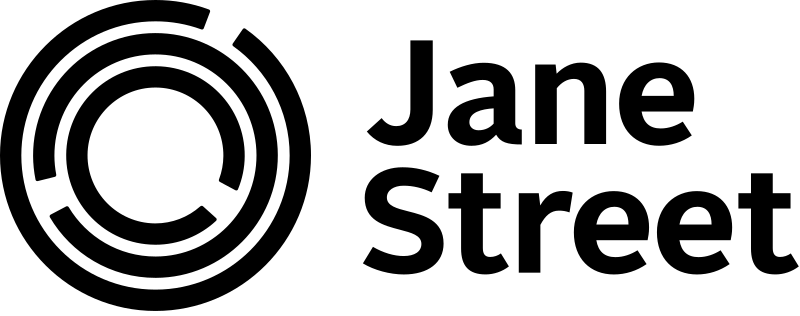
\includegraphics[scale=0.35]{./images/argb.png}
\end{center}

\section{Derivation of the Gradient for Non-linear Programming}

We optimize for the variable $\theta$. We get following base function.
\begin{gather*}
    X_{t + 1} = X_{t} + -\theta(X_{t} - \mu)e + \mathcal{N}(0, \sigma^{2}) \\
\end{gather*}
We must get the objective function which is thre mean squared error in terms of $\theta$.
We consider the the values to be in a pre-computed list $\mathcal{X}$, where $\mathcal{X}_{1}, \mathcal{X}_{2}, \dots, \mathcal{X}_{n} \in \mathcal{X}$
\begin{gather*}
    MSE = \frac{1}{T} \sum_{i = 1}^{T} \mathcal{X}_{i} = \frac{1}{T} \sum_{i = 1}^{T} X_{i} + -\theta(X_{t} - \mu)e + \mathcal{N}(0, \sigma^{2})
\end{gather*}

\section{Least Squares Regression for Mean-reverting Parameter}
\begin{gather*}
    \mathcal{X}_{t + 1} = \mathcal{X}_{t} - \theta (X_{t} - \mu)e + \mathcal{N}(0, \sigma^{2}) \\
    \mathcal{X}_{t + 1} - \mathcal{X}_{t} - \mathcal{N}(0, \sigma^{2}) = -\theta (X_{t} - \mu)e  \\
    \frac{- \mathcal{X}_{t + 1} + \mathcal{X}_{t} + \mathcal{N}(0, \sigma^{2})}{e(X_{t} - \mu)} = \theta
\end{gather*}

For now, we can disregard the normally-distributed Wiener process term.
Have to use Ito's Lemma.

\end{spacing}
\end{document}
